\documentclass[aps,prl,reprint,groupedaddress]{revtex4-1}
\usepackage{graphicx}    % Required for inserting images.
\usepackage{amsmath,amssymb,gensymb}  % Advanced math formatting.
\usepackage{float}  % Required to force figure position.
\usepackage{lipsum} % For dummy text.
\usepackage{hyperref}
 

\begin{document}

\title{Calibration of a Three-dimensional Muon Detector Based on Scintillator Binary Optical Encoding\\[0.5ex] \small Team Dawson Technicolor}

\author{Milo Belarbi}
\author{David Birnbaum}
\author{Tykhon Byshkin}
\author{Matvey Chirchikov}
\author{Danah Dézémé}
\author{Arij Mohamedi} 
\author{Evan Parasol}
\author{Leandro Perez Moran}
\author{Ari Polterovich}
\author{Tian Yi Xia}
\author{Chun On Yu}
\author{Aljoscha Ziegler}
\author{Manuel Toharia}
\altaffiliation{Teacher}
\author{Joel Trudeau}
\altaffiliation{Teacher}

\affiliation{Dawson College, Montreal, Quebec, Canada}
\date{April 10, 2025}

\maketitle



%\begin{multicols}{2}

\section{Introduction}
At any given moment, there are muons raining down on us at a rate of approximately 1 muon per square centimeter per minute [1]. Traditionally, they are observed with the use of a spark chamber. However, building a spark chamber is a technical challenge, especially for high school students. We wanted to create a simple and easily reproducible way of observing muons, which is what led us to develop our three-dimensional scintillator-based detector, a.k.a. The Scintillating Chamber. Although we have developed the detector’s software and hardware components, precise calibration would require exposure to a controlled muon beam. Access to CERN’s world-class facilities would allow us to validate our detector’s performance and refine its accuracy. It would also provide invaluable insights into innovative techniques that would contribute to the broader field of particle detection technology. We hope to collaborate with peers and experts at CERN to deepen our comprehension of physics concepts through real-world applications. We are also committed to inspiring other young Canadian scientists by sharing our experiences and findings through outreach activities. An opportunity to conduct our experiment at CERN would be a pivotal step in this journey. We hope that our design can be used in physics classrooms around the world to assist science education and communication. Our team hopes to continue development to enhance our detector for these purposes, adding a timing device to measure the energy of the detected particles, and creating a better user interface for easier use in classrooms.


\section{Design}
\lipsum[1]



\vspace{40mm}
\section{Results}
\lipsum[1]


%\clearpage

\section{Experimental Proposal}
\lipsum[1]


\section{Outlook}
We have fully developed the detector’s software and hardware components on our own. Therefore, precise calibration would require exposure to a controlled muon beam. Further, a controlled muon beam would permit us to test out features we are currently developing such as measuring the detection time and using a time-over-threshold system to find the energy of muons passing through the detector. Access to CERN’s facilities would allow us to validate our detector’s performance and refine its accuracy.

The confirmation of the viability at CERN of our safety-oriented detector design allows for open-sourcing, along with physics classroom outreach—projects with which we align. We believe that getting this detector ready for research will inspire more students to design their own particle physics experiments.


%TC:ignore
\section{Community outreach}
Women, though largely unrecognized, have played a great role in the development of modern science. Marie Curie, Ada Lovelace, Katherine Johnson, and many others have been role models for generations of scientists. Our team at Dawson TECHNICOLOR firmly believes that part of promoting science education is promoting the inclusion of women and other marginalized groups. As such, we are currently working with Dawson STEMM FEM, a local club, to create talks and participate in events that will hopefully encourage many young women to join the beautiful field of physics and of science as a whole.

Furthermore, The Scintillating Chamber is set to be presented in May at Dawson’s ScienceFest. This event consists of a fair where a myriad of scientific projects are introduced to the student body. This opportunity will allow us to make particle physics more accessible and easier to grasp while sharing our unwavering passion.

%\end{multicols}

% Section: Acknowledgements
%\clearpage
\section{Acknowledgments}
We would like to sincerely thank Dr. Manuel Toharia for his dedication to the High Energy Particle Physics group at Dawson, for his captivating lectures and for his guidance throughout our project. We are incredibly grateful to McGill University Professor Dr. David Hanna for his invaluable advice and for graciously letting us use his scintillator block as well as McGill University Professor Dr. François Corriveau for his guidance. We express our sincere appreciation to Université de Montréal technician Dr. Nikolai Starinsky for his scintillator cutting advice. This project would not have been possible without the Dawson Foundation’s Student Academic Growth and Enrichment Fund, whose grant provided money with which we bought power tools, safety equipment, and electronics. Finally, we would like to express our gratitude to Dawson College for offering us a wonderful learning environment that allowed us to flourish and engage in science activities that we are passionate about. 


\clearpage
\section{Appendices}
\begin{figure} [h]
    \centering
    \includegraphics[scale=0.5]{figures/fig5.png}
    \caption{\textbf{Top:} Signal acquisition circuit. \textbf{\textit{Left:}} Low-noise 5\,V power supply for all SiPM PCB boards (TPS7A470, $4\,\mu\text{V}_\text{RMS}$). \textbf{\textit{Middle:}} 24-channel digital signal reader with FPGA (ICE40HX1K), 5\,V to 3.3\,V level shifters, and indicator LEDs associated with each SiPM sensor. \textbf{\textit{Right:}} Breadboard: Arduino Nano for serial data communication over USB to the computer, and STM32F103C for clock signal generation. \textbf{Bottom left:} Work in progress FPGA detector module. \textbf{Bottom right:} Manual soldering of individual wires for the 24 LED indicators.}
    \label{fig5}
\end{figure}


\begin{figure}[h] 
    \centering 
    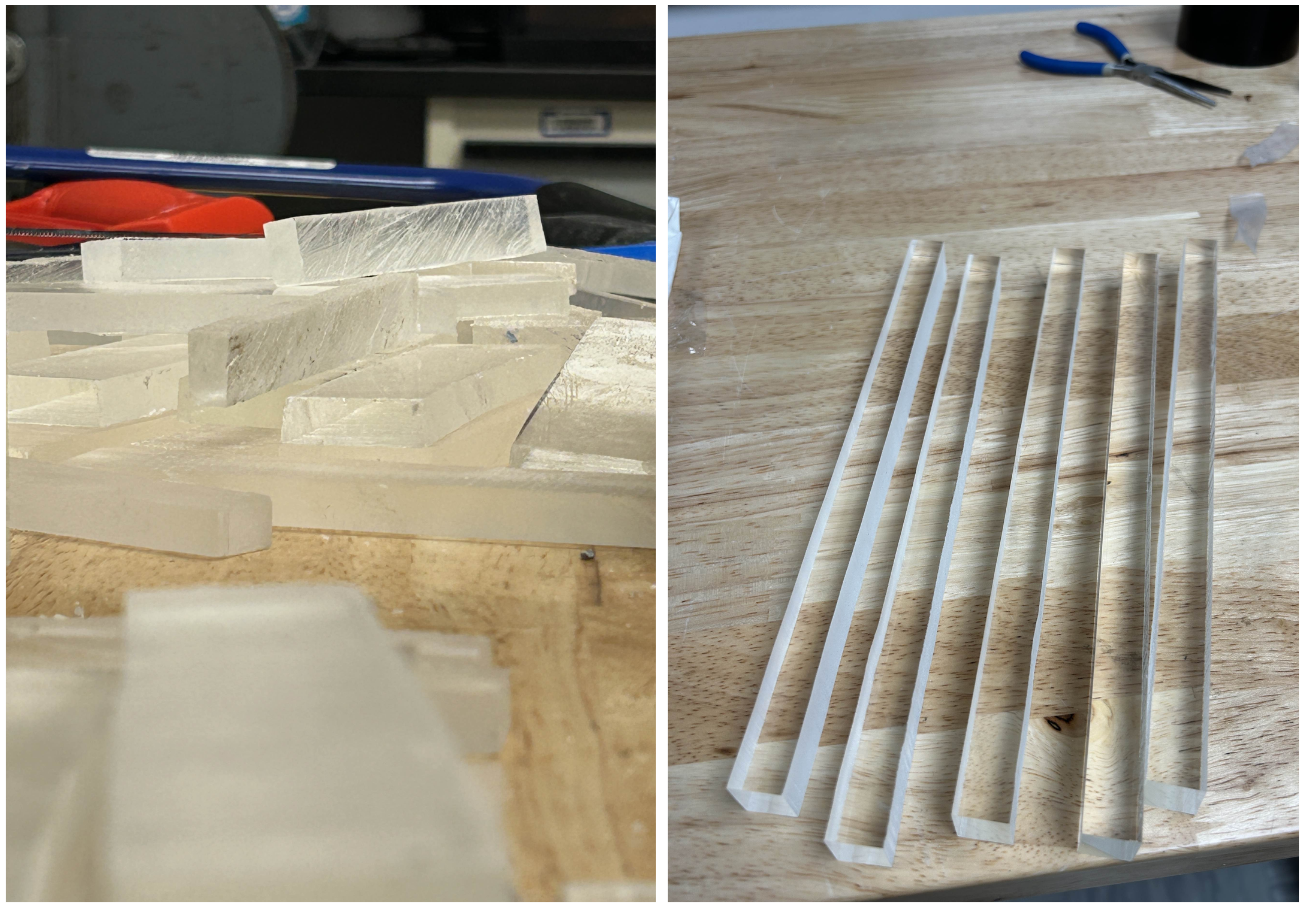
\includegraphics[scale=0.6]{figures/fig6.png}
    \caption{Scintillator rods cut with a bandsaw from a larger
scintillator block. Two $500\times250\times30$ mm BC408 PVT scintillators were graciously offered to us by McGill Professor Dr. David Hanna\textemdash which we then proceeded to cut and polish manually.}
    \label{fig6}
\end{figure}





\begin{thebibliography}{99}
% \cite{Spectrum of CRM}
\bibitem{Spectrum of CRM}
Gardner, M., et al., "The Momentum Spectrum of Cosmic Ray Muons near Sea Level in the Momentum Range 0.4--10 GeV/c." IOPScience. Accessed March 2022,
\url{https://iopscience.iop.org/article/10.1088/0370-1328/80/3/314/pdf}.

% \cite{hyperphysics}
\bibitem{hyperphysics}
Hyperphysics, "Atmospheric Muons." Georgia State University. Accessed March 2022,
\url{http://hyperphysics.phy-astr.gsu.edu/hbase/Particles/muonatm.html}.

% \cite{atmospheric muon}
\bibitem{atmospheric muon}
CERN, "Cosmic Rays: Particles from Outer Space." Accessed March 2022,
\url{https://home.cern/science/physics/cosmic-rays-particles-outer-space}.

\bibitem{pdg}
K.~Nakamura \textit{et al.} [Particle Data Group], J. Phys. G \textbf{37}, 075021 (2010),
doi:10.1088/0954-3899/37/7A/075021,
\url{https://pdg.lbl.gov/2011/reviews/rpp2011-rev-cosmic-rays.pdf}.



\bibitem{agc}
Kuttner, P. The rope memory: a permanent storage device. {\em Proceedings Of The November 12-14, 1963, Fall Joint Computer Conference}. pp. 45-57 (1963), \url{https://doi.org/10.1145/1463822.1463829}


\bibitem{wls}Worstell, W., Doulas, S., Johnson, O. \& Lin, C. Scintillator crystal readout with wavelength-shifting optical fibers. {\em Proceedings Of 1994 IEEE Nuclear Science Symposium - NSS'94}. \textbf{4} pp. 1869-1873 vol.4 (1994)
\url{https://dl.acm.org/doi/pdf/10.1145/1463822.1463829}


\end{thebibliography}
%TC:endignore

\end{document}